\chapter{Example section}\label{ch:example}

This document demonstrate the use of figures, references, SI units, glossary, math notation, lists, and otherwise relevant formatting specifications. Paragraphs are typically separated using \texttt{\textbackslash medskip}.\medskip

\begin{figure}[H]
    \centering
    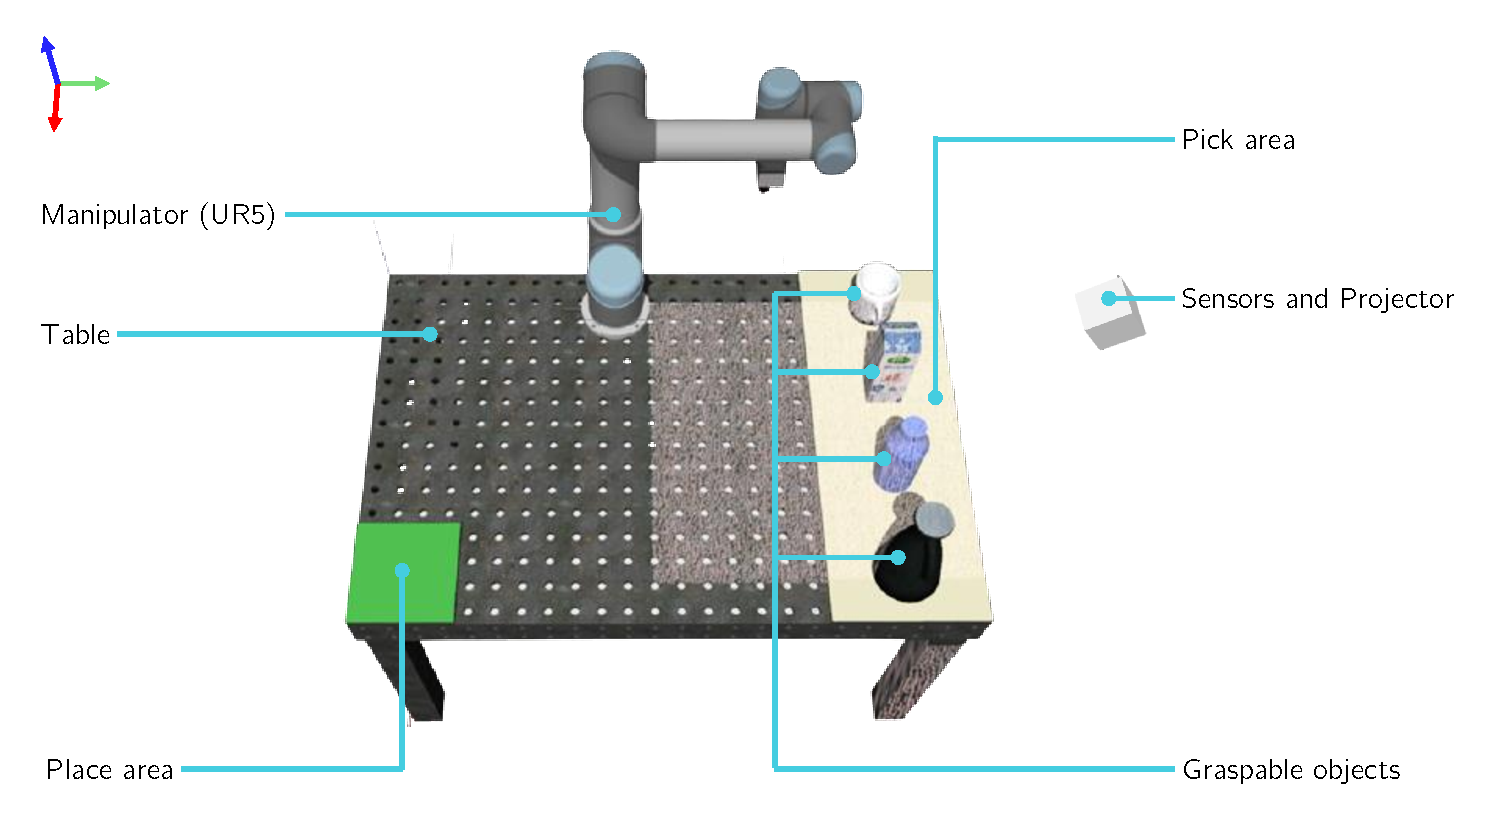
\includegraphics[width=.6\linewidth]{chapters/example/fig/figure.pdf}
    \caption{An example image using \acrlong{acronym-label}.}
    \label{fig:example-figure}
\end{figure}

To exemplify math notation, consider the mapping between the joint configuration of a robot
%
\begin{equation}
    \vec{q} = \rvec{q_1 & q_2 & \dots & q_n}\T,
    \label{eq:jnt-config}
\end{equation}

and \gls{glossary-label}, given as a homogeneous transformation
%
\begin{equation}
    \renewcommand{\arraystretch}{1.2}
    \tf{A}{B} = \begin{bmatrix}
        \tf[R]{A}{B}         & \tf[t]{A}{B} \\
        \vec{0}^{1 \times 3} & 1 
    \end{bmatrix},
\end{equation}

where \tf[R]{A}{B} and \tf[t]{A}{B} is the rotation and translation, respectively, from frame $\{A\}$ to frame $\{B\}$, denoted using a homogeneous transformation matrix $\mat{T}(\vec{q}) \in \mathbb{R}^{4 \times 4}$ as a function of the joint configuration in \eqref{eq:jnt-config}, as described in \cite{robotics-book}.\medskip

Complex table/figure hybrids with aligned captions and functioning labels can be implemented using \texttt{minipage}, as shown in \tabref{tab:example-table} and \figref{fig:example-plot}. Use \fakecite as a placeholder for citations.

\begin{center}
    \renewcommand{\arraystretch}{1.2}
    \begin{minipage}{.4\linewidth}
        \vspace{-10pt}
        \centering
        \begin{tabular}{|l|c|c|c|}
        \hline
        \diagbox[width=5.5em, font=\footnotesize\bfseries]{Method}{Pose} & 1 & 2 & 3 \\ \hline
        Linear    & \SI{18.97}{\second} & \SI{20.35}{\second} & \SI{22.85}{\second} \\ \hline
        Parabolic & \SI{13.66}{\second} & \SI{14.93}{\second} & \SI{17.33}{\second} \\ \hline
        \end{tabular}%
    \end{minipage}%
    \hfill%
    \begin{minipage}{.55\linewidth}
        \vspace{0pt}
        \centering
        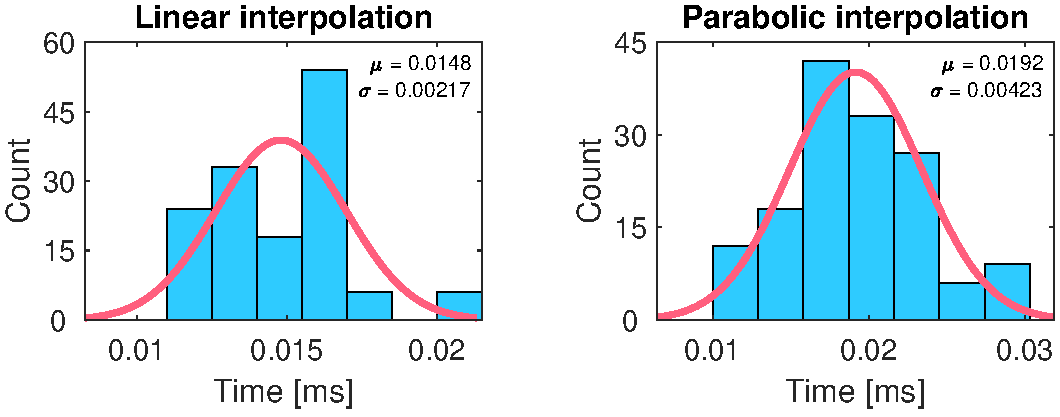
\includegraphics[width=.95\textwidth]{chapters/example/fig/plot.pdf}
    \end{minipage}%
    %    
    \vspace{15pt}
    %
    \begin{minipage}[t]{.4\linewidth}
        \vspace{0pt}
        \captionsetup{type=table}
        \captionof{table}{Trajectory durations of the interpolation-based trajectory generation methods.}
        \label{tab:example-table}
    \end{minipage}%
    \hfill%
    \begin{minipage}[t]{.55\linewidth}
        \vspace{0pt}
        \captionsetup{type=figure}
        \captionof{figure}{Average planning time for each of the interpolation-based trajectory generation methods.}
        \label{fig:example-plot}
    \end{minipage}%
\end{center}

For numbers, units and ranges, the \texttt{siunitx} package is used, which allows to express a number \num{10}, a range of \SIrange{5}{6}{\second}, or a SI unit of \SI{5.73 \pm 1.09}{\second}. Inline row-vectors (with the transpose symbol) can be written as $\vec{a} = \rvec{\vec{a}_p & \vec{a}_o}\T$, where as parentheses can be automatically written using $\qty(a, b)$ or $\qty{\frac{a}{b}, c}$. Also, shorthands for \mat{A}\inv, \mat{A}\pinv and \mat{A}\T.\medskip

\glsresetall